%----------------------------------------------------------------------------------------
%----------------------------------------------------------------------------------------
%----------------------------------------------------------------------------------------
%Result Part 1: 1D SOMs
%----------------------------------------------------------------------------------------
%----------------------------------------------------------------------------------------
%----------------------------------------------------------------------------------------
\section{One-Dimensional Self-Organizing Maps}
    \label{Sec: 1d_cluster}
%Why 1D maps are useful
    The purpose of  exploring the M31 data with 1D maps is to monitor the general behaviour of the data. 
    One-dimensional SOMs can have the minimum number of clusters, $1\times2$, up to the highest number of clusters possible (infinity). %Els asked what is maximum possible #
    In a small sample like ours, smaller grid SOMs are very useful to find correlations that cannot be found without  clustering the data.
    On the other hand, larger grid 1D SOMs are a helpful tool to get quick insight into the data.

    \subsection{Clustering M31 Data}

        In order to monitor how the data behave, we created SOMs with two to fourteen neurons (Fig.~\ref{fig: M31_nets_1d}).
        The $1\times2$ network (Fig.~\ref{fig: M31_net_1by2}) shows how the M31 data can be divided into two broad categories.
        The $1\times14$ network (Fig.~\ref{fig: M31_net_1by14}) is the first network in which all the regions in M31 are completely separated.
        In the higher network sizes, regions have more space to be separated based on their differences. In going from the $1\times2$ to the $1\times14$ network the distance between M31 regions increases, until they are completely separated. 
        
        Fig.~\ref{fig: M31_net_1by2} shows that by forcing the regions in the M31 to be divided into two groups, regions 1, 2, 9 and 10 (shown in Fig.~\ref{fig: regions in m31}) occupy one neuron and the other regions occupy the other one.
        The medium grey colour between two neurons indicates that there are some similarities between two groups, but they are not very similar. 
        By increasing the size of the neurons to three, in Fig.~\ref{fig: M31_net_1by3}, we can see that region 2 separates itself from the other regions and occupies the middle neuron.
        The white colour between the two left neurons suggests that the regions which occupy these neurons are very similar to each other, while the black colour between the two right neurons indicates otherwise.
        
        %%%Talking about four right regions
        \cite{Dim15} showed that regions 1, 2, 9, and 10 have higher PAH fluxes compared to the other regions (fig.~5 in \citealt{Dim15}). 
        These regions also have relatively high intensities in all the mid-infrared and far-infrared bands and have high dust luminosity and dust mass.
        The higher values for these quantities could be the reason that these four regions become separated from the others in the $1\times2$ network.
        Regions 1 and 9 are in the 10~kpc ring, region 2 is slightly out of the 10~kpc ring and region 10 is in the bulge of M31; however, regions 3 to 8 are located out of the inner ring or the 10~kpc ring (Fig.~\ref{fig: regions in m31}).   
        The differences in their positions account for their difference in input parameters.
        Since region 10 is located in the bulge of M31 and has high surface brightness for most of the input values, regions 1, 2, and 9 to gradually move towards other regions and away from region 10 in the higher grid SOMs.
       
    \begin{figure}
    \begin{subfigure}[b]{0.5\textwidth}
        \centering
        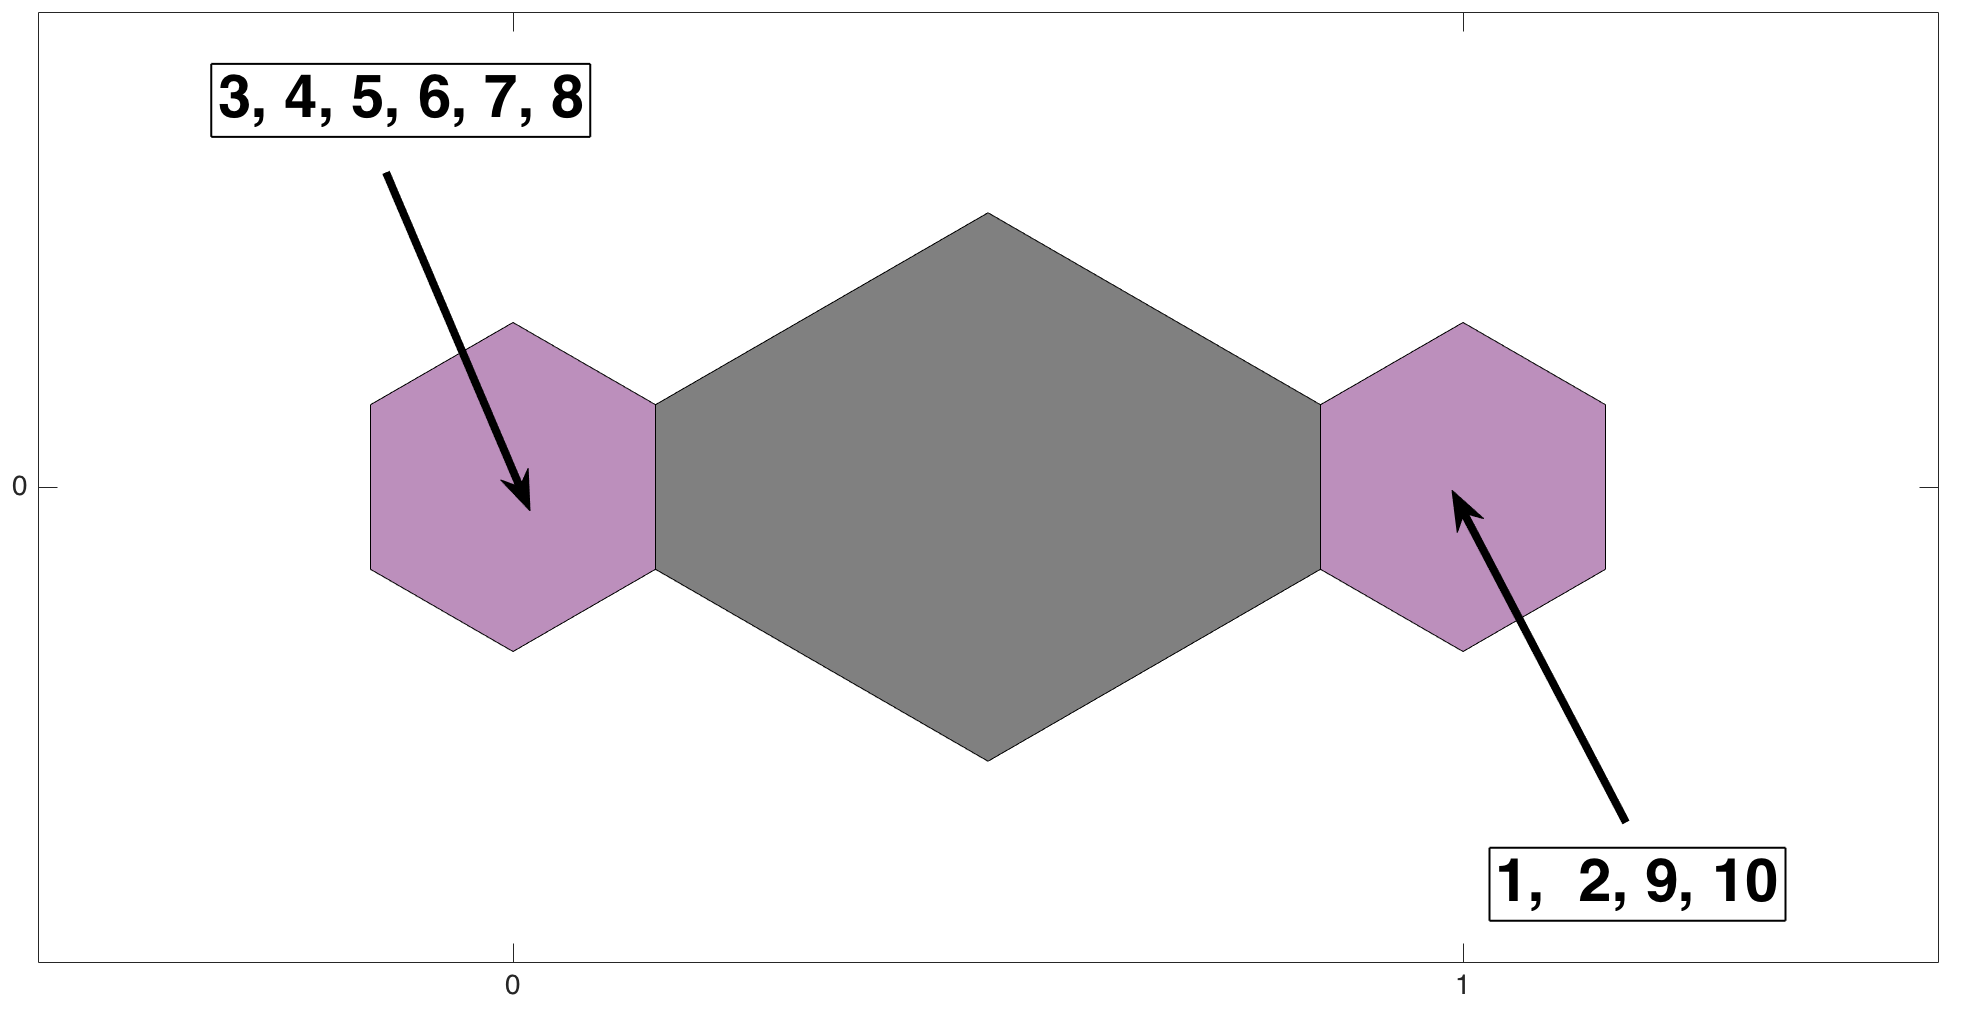
\includegraphics[width=\textwidth]{../images0.01/M31/1D/combine_1D_1by2_all.png}
        \caption{$1\times2$~network}
    \label{fig: M31_net_1by2}
    \end{subfigure}
    \hfill
    \begin{subfigure}[b]{0.5\textwidth}
        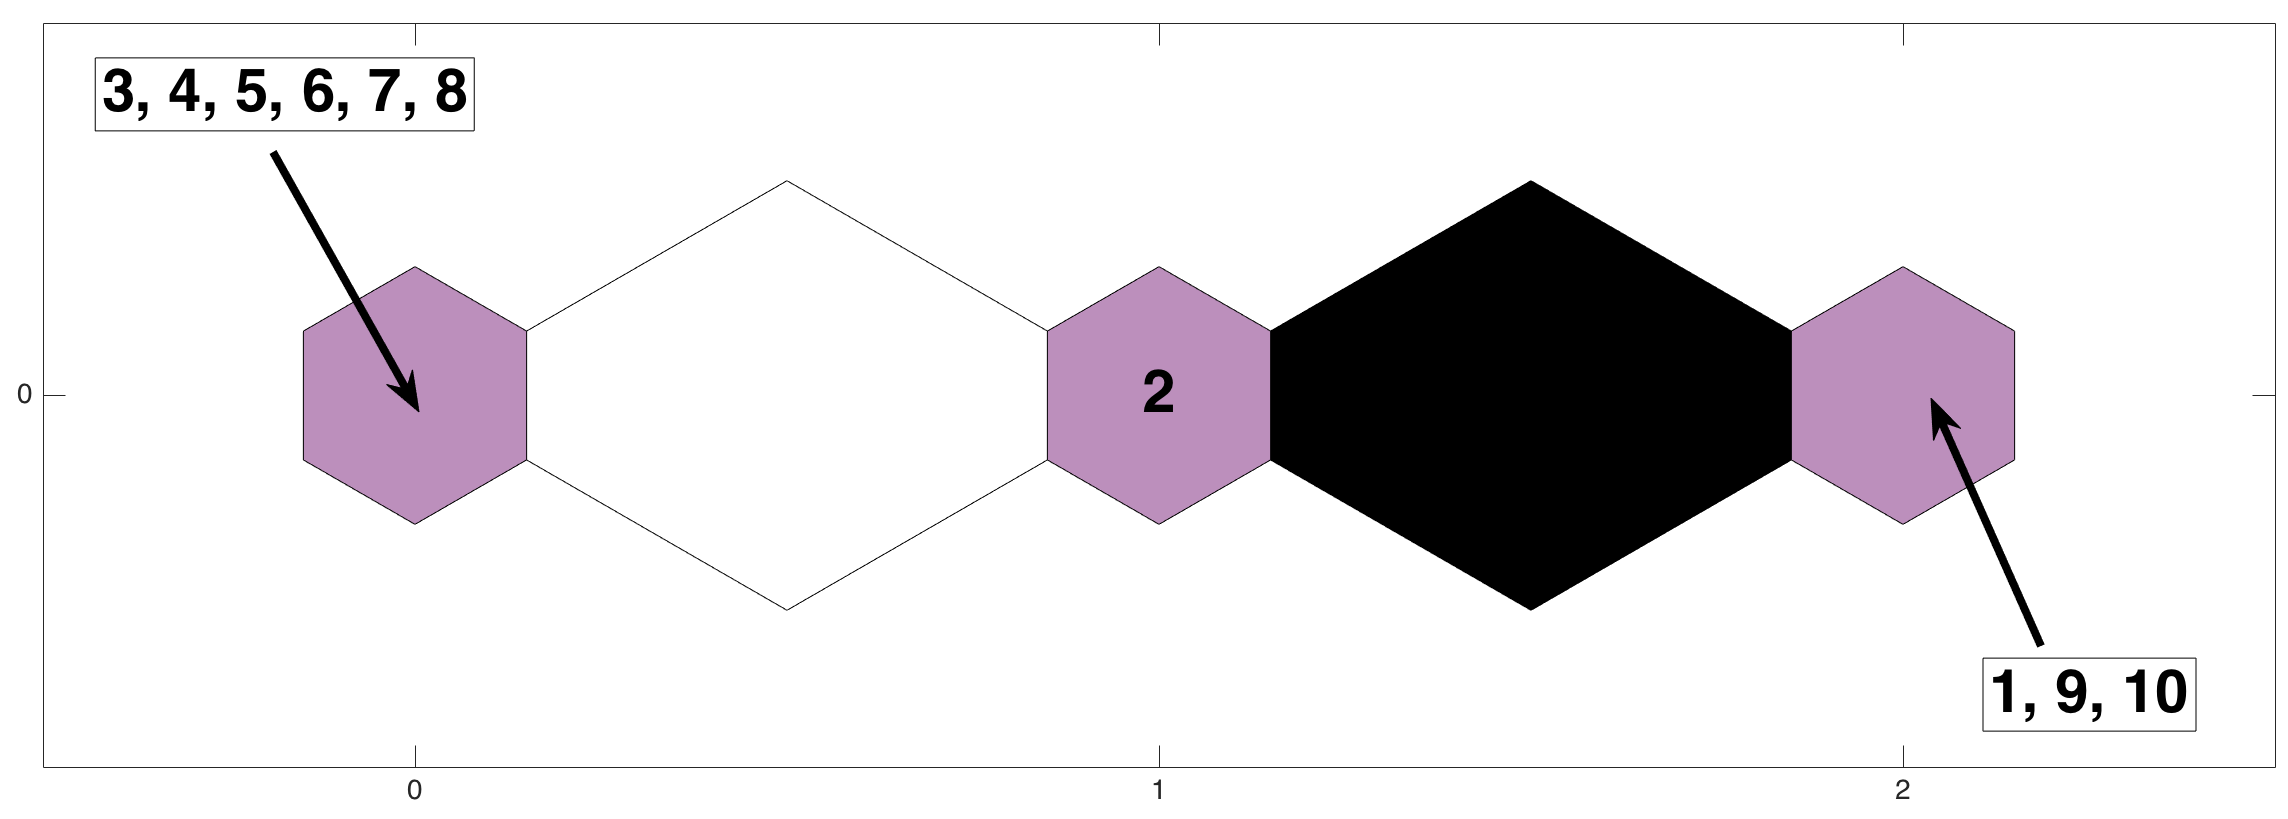
\includegraphics[width=\textwidth]{../images0.01/M31/1D/combine_1D_1by3_all.png}
         \caption{$1\times3$~network}
        \label{fig: M31_net_1by3}
    \end{subfigure}
    \hfill
    \begin{subfigure}[b]{0.5\textwidth}
        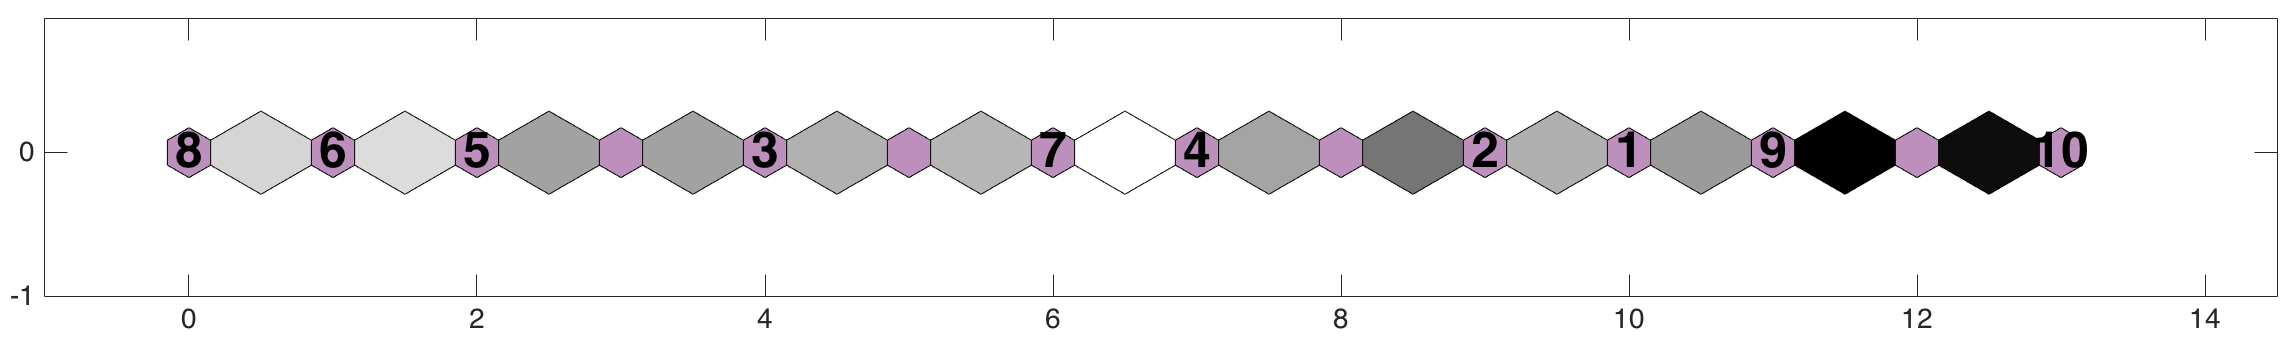
\includegraphics[width=\textwidth]{../images0.01/M31/1D/combine_1D_1by14_all.png}
        \caption{$1\times14$~network}
        \label{fig: M31_net_1by14}
    \end{subfigure}
   \caption[One-dimensional self-organizing map of M31 data]{SOM of the M31 data from $1\times2$, $1\times3$~and $1\times14$~grids. The axes show the position of the neurons. The purple hexagonal shapes represent the neurons. The grey scale colours show the differences between weight of the neurons, with white as the minimum difference and black as the maximum. The numbers in the plot show the M31 regions located in each neuron.}
   \label{fig: M31_nets_1d}
    \end{figure}
    

        %%Network 1by14
        The network with 14 neurons, in Fig.~\ref{fig: M31_net_1by14}, is the first network that has no neuron occupied by more than one M31 region.
        In a larger-grid SOM, the network pays more attention to smaller details and differences in the input data.
        Therefore, since at least 14 neurons are needed to separate all 10 regions in M31, we can conclude that some of the regions have very small differences.
        Regions that are located in similar areas (e.g. spiral arms, bulge, and 10 kpc ring) in M31, like regions 7 and 4 (see Fig.~\ref{fig: regions in m31}), are most likely to have more similarities with each other.
        In Fig.~\ref{fig: M31_net_1by14}, the right-most neuron is occupied by region 10.
        Two black colours between this region and the others indicate the large differences between this neuron and the other ones.
        Region 10 is located in the bulge of M31, and is physically separated from the other regions, which are mostly located around the inner or outer rings.
        The SOM shows that this region has completely different input values from the others: most of the values for region 10 are much higher than for the other regions, which is the main reason for its isolation.
        Region 8 occupies the right-most neuron in this network, suggesting that this region has the most differences from region 10.
        
    \subsection{Inside the Two Neuron Network}
        \label{sec: inside_the_2_neurons}
        Using self-organizing maps, we can identify hidden subgroups in our samples. 
        Each of these subgroups separates for a reason.
        This reason can vary from having higher values in some specific properties, as discussed in Section~\ref{Sec: 1d_cluster}, to some unknown correlations between data that cannot be seen in other groups or in the galaxy as a whole.
        To investigate the latter, we show in Fig.~\ref{fig: cor_cluster1} the Pearson correlation coefficients for the inputs from regions 3 to 8, which were clustered together in the $1\times2$ and $1\times3$ networks (see Figs.~\ref{fig: M31_net_1by2} and ~\ref{fig: M31_net_1by3}).
        
        \begin{figure*}
        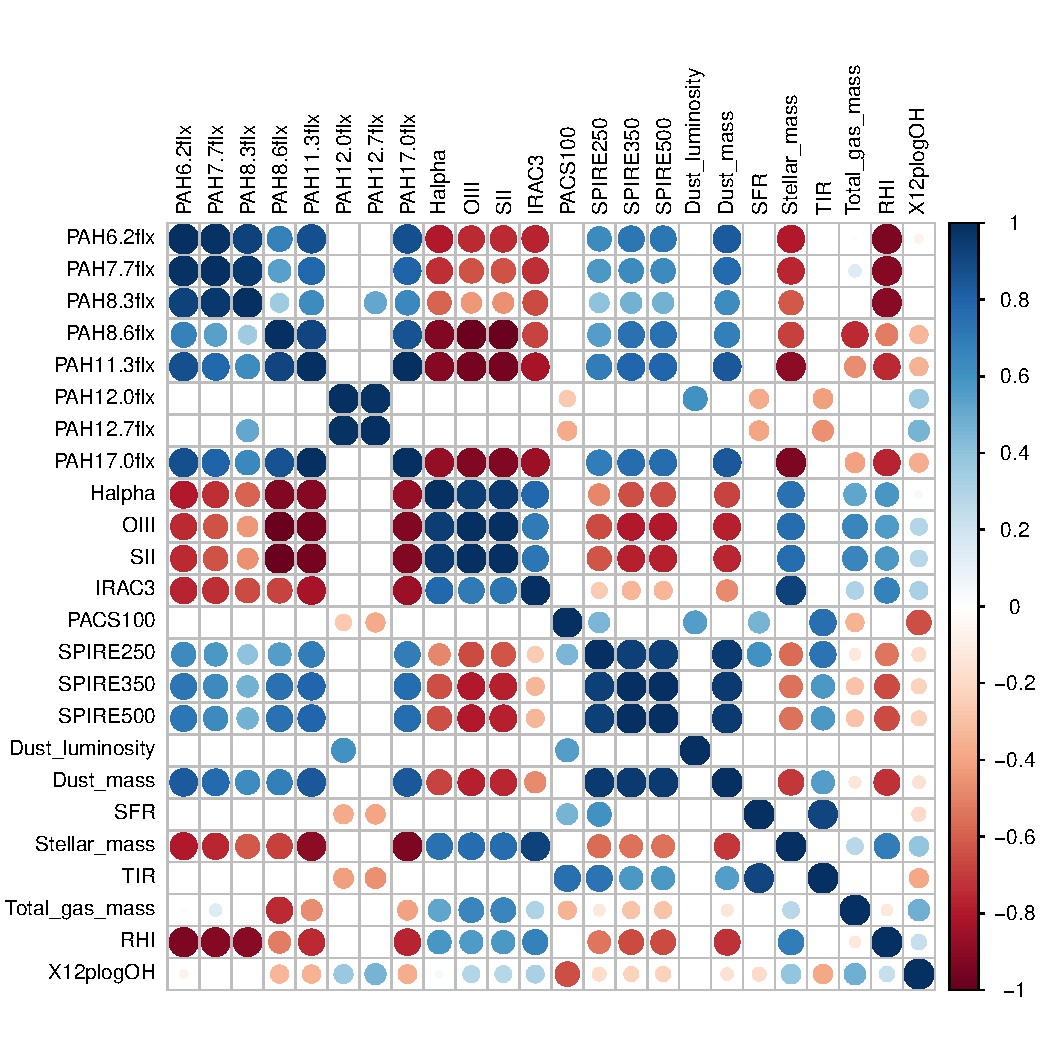
\includegraphics[width=\textwidth]{../images0.01/cor_plots/M31_derived_3_to_8_core_plot_for_paper.pdf}
        \caption[Pearson correlation coefficients for data from the clustered regions in M31]{Same as Fig.~\ref{fig: cor_all}, but here we used data from regions grouped in the left sides of Figs.~\ref{fig: M31_net_1by2} and ~\ref{fig: M31_net_1by3}. }
          \label{fig: cor_cluster1}
        \end{figure*}
        
       
        Comparing the correlation coefficient plots for all 10 regions in M31 (Fig.~\ref{fig: cor_all}) and for the clustered data (Fig.~\ref{fig: cor_cluster1}) shows the differences between all 10 regions and clustered data and why regions 3 to 8 become separated from the other regions.
        The main features that differentiate these two plots are the anti-correlations between PAH features and RHI, stellar mass, \halpha, \sii, \oiii, and IRAC~5.8~$\mu$m~emission.
        Additionally, for the PAH fluxes in Fig.~\ref{fig: cor_cluster1}, there are no significant correlations with PACS~100~$\mu$m, L$_\mathrm{dust}$, L$_\mathrm{TIR}$, SFR, or metallicity.
        The PAH fluxes correlate with the SPIRE emission, but to a lesser extent than for the data from all regions.
        
        \cite{Calzetti10} mentioned that with increasing RHI in regions, metallicity and PAH equivalent widths decrease. 
        \cite{Dim15} investigated the correlation between PAHs features and both metallicity and RHI using the equivalent width of the 8~$\mu$m (combination of 7.7, 8.3, and 8.6~$\mu$m components) and the 7.7 and 11.2~$\mu$m features.
        They did not see any relations between PAHs and metallicity or RHI for 10 regions in M31.
        In Fig.~\ref{fig: cor_all}, we show that all the PAH fluxes correlate with metallicity, and PAH fluxes in the 7.7, 8.3 and 17.0~$\mu$m bands weakly anti-correlate with RHI.
        However, in Fig.~\ref{fig: cor_cluster1}, there is no correlation between the PAH fluxes and metallicity, but all of them strongly anti-correlate with RHI.
        \cite{Dim15} argued that the absence of (anti)-correlation between the PAH features and metallicity and RHI was related to a lack of data in low-metallicity regions.
        Although data from more regions would improve the results, our analysis shows that clustering data would show the missing (anti)-correlations.
        For example, for both clusters in Fig.~\ref{fig: M31_net_1by2},
        we can see anti-correlations between PAHs and RHI, but each of them has a different slope which removes the anti-correlation over all 10 regions. 
        
        Correlations between PAH features and SFR, and L$_\mathrm{TIR}$ are well-studied~\citep[e.g.][]{Peeters04,Tielens08}. 
        Many groups have used PAH features as a tracer of SFR by finding correlations between 
        PAH emission and SFR derived from extinction-corrected \halpha~\citep[e.g.][]{Calzetti07,Khramtsova13,Shipley16}.
        These correlations are seen in Fig.~\ref{fig: cor_all}, when we considered the data from all regions, but not in Fig.~\ref{fig: cor_cluster1} when considering the clustered data.
        Note that, since there are only 6 regions in the clustered data, even one outlier in the data may cause the correlation coefficient to become insignificant.
        Further analyses show that the absence of correlations between PAH fluxes and SFR is because of one outlier: region 6. Region 6 is located in a FUV-bright region, which breaks the correlations. 
        When we disregard this region, high correlations between 6.2 to 17.0~$\mu$m~PAHs and SFR (and L$_\mathrm{TIR}$) reappear.
        
     
        Strong anti-correlations between 6.2 to 17.0~$\mu$m~main PAH features and RHI, stellar mass, \halpha, \sii, \oiii, and IRAC~5.6~$\mu$m~emission in Fig.~\ref{fig: cor_cluster1} were not seen in Fig.~\ref{fig: cor_all} (even if we ignore the outlier values).
        Anti-correlations between PAH features and the \halpha, \sii, and \oiii~emission could be the result of one of the following. 
        First, the optical data are not corrected for dust extinction.
        The PAH features correlate with the amount of dust while \halpha~emission anti-correlates with the amount of dust due to extinction as suggested by \cite{Calzetti94}.
        Therefore, higher PAH fluxes imply higher dust abundance and less \halpha~emission, and the same holds for \sii~and \oiii~emission.
        Second is the possible effect of the structure of the observed regions.
        If the observed regions are located near the edge of \hii~regions we would expect to see more PAH and less \halpha~emission. 
        The anti-correlations between 6.2 to 17.0~$\mu$m~PAH features and RHI have been seen in other studies, as well~\citep[e.g.][]{Wu06, Gordon08,Calzetti10,Dim15}. 
        \cite{Wu06} suggested these anti-correlations could be the result of PAH destruction due to a high amount of harder radiation (thus higher RHI).
        On the other hand,~\cite{Gordon08} argued that the harder radiation could make the photodissociation regions (PDRs) smaller.
        The PAH features are mostly coming from the PDRs that are surrounded by \hii~regions, and the PAH features' underlying continuum emission is from the \hii~regions.
        Therefore, the lower flux of the PAH features could be the result of the smaller size of PDRs.%Els: If you have an harder radiation field, you destroy your smaller PAHs. Hence, simply a harder RHI does not argue for a smaller PDRs being more plausible. 
        The latter reason, which could also describe the anti-correlation between PAH features and \halpha~emission, seems to be the more probable one. 
        
        The strong anti-correlation between PAHs and stellar mass suggests that, a higher stellar mass decreases PAH emission. 
        In observations of M33,~\cite{Calapa14} showed that the 8/250~$\mu$m luminosity ratio correlates with 3.6~$\mu$m emission, which translates to stellar mass, %Els: I'm unfamiliar with the details of this translation. But if you look at individual HII regions or starforming complexes, I would think that the 3.6um flux is not dominated by the stellar light as the stars are too hot to have a large fraction of emission at these wavelengths?
        and conclude that the PAH emission traces the old stellar population.
        In Fig.~\ref{fig: cor_cluster1}, we see a weak anti-correlation between SPIRE 250~$\mu$m emission and the stellar mass.
        We see no correlation between 8/250~$\mu$m luminosity and stellar mass, either in the clustered data or in all 10 regions.

        To test that whether the anti-correlation between stellar mass and PAH emission is the result of the destruction of PAHs in high stellar mass regions, or that high stellar mass obscures PAH emission, we compared PAH abundance with stellar mass for the clustered regions.
        The ratio of 8/24~$\mu$m emission, which can be considered as a proxy for PAH abundances~\citep[e.g.][]{Sandstrom10,Khramtsova13}, does not anti-correlate with stellar mass for either the clustered data or all 10 regions.
        Therefore, we conclude that in our sample, stellar mass does not cause the destruction of PAHs.
        
        The anti-correlation between stellar mass and PAHs could be result of the position of the regions within M31.
        Regions 5, 6, and 8 are located in the stellar disk of the galaxy and have relatively high stellar mass and faint PAH emission. 
        According to~\cite{Dim15}, regions 5 and 8 are the only two regions in thesample that do not include an \hii~region, which could be the reason for the faint PAH emission for these regions.
        Regions 4 and 7 have similar quantities for both stellar mass and PAHs and region 3 has high PAHs and low stellar mass.
        Without data from more regions in M31, we cannot confidently say that higher stellar mass decreases PAH fluxes.
        
        
       Regardless of the fact that some of the (anti)-correlations in Fig.~\ref{fig: cor_cluster1} might have physical meaning, we have to mention that we only used 6 regions to calculate these correlation coefficients.
       The number of data points is not high enough to yield a strong conclusion about PAH properties in M31.
       However, we can conclude that since the correlation coefficients derived from the clustered data (Fig.~\ref{fig: cor_cluster1}) differ from the correlation coefficients derived from the data from all 10 regions (Fig.~\ref{fig: cor_all}), the SOM separated a hidden cluster of the data which has different properties.
        
        
        